\section{Durchführung}
\label{sec:Durchführung}
Der Versuch besteht aus einer Kupfer-Röntgenröhre mmit einem LiF-Kristall und einem Geiger-Müller-Zählrohr.
Der Versuchsaufbau ist in \autoref{fig:aufbau} abgebildet.
\begin{figure}[H]
    \centering
    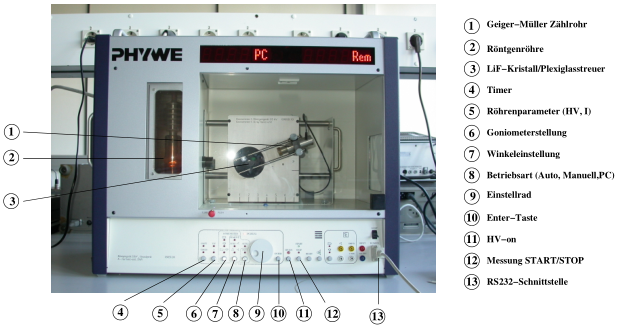
\includegraphics[width = 0.7 \textwidth]{data/aufbau.png}
    \caption{Versuchsaufbau zur Messung von Röntgenemission und -absorption \cite{Anleitung602}.}
    \label{fig:aufbau}
\end{figure}
Als erstes wird in einem Messbereich von $\SIrange{5}{26}{\degree}$ das Emissionsspektrum der Kupfer-Röntgenröhre aufgezeichnet. Es wird ein Winkelzuwachs von 
$\upDelta \alpha = \SI{0,}{\degree}$ mit einer Integrationszeit von $\upDelta t=\SI{5}{\second}$ gewählt. \newline
In einem zweiten Versuchsschritt wird das Absorptionsspektrum verschiedener Stoffe aufgenommen und der Bragg-Winkel bestimmt.
Dazu wird vor das Geiger-Müller-Zählrohr Blenden mit Absorbern unterschiedlicher Elemente gesteckt. Es werden dabei alle möglichen Spektren aufgenommen, zu denen Stoffe zur Verfügung stehen.
Die Messungen wurden mit einer Beschleunigungsspannung von $U_{\text{B}} = \SI{35}{\kilo\volt}$ gemessen.